\documentclass[12pt,twoside]{article}   
\usepackage{light}
\usepackage{graphicx}
\usepackage{verbatim}

\newcommand{\hint}[1]{({\it Hint: #1})}
\newcommand{\card}[1]{\left|#1\right|}
\newcommand{\union}{\cup}
\newcommand{\lgunion}{\bigcup}
\newcommand{\intersect}{\cap}
\newcommand{\lgintersect}{\bigcap}
\newcommand{\cross}{\times}

\hidesolutions
%\showsolutions

\newlength{\strutheight}
\newcommand{\prob}[1]{\mathop{\textup{Pr}} \nolimits \left( #1 \right)}
\newcommand{\prsub}[2]{\mathop{\textup{Pr}_{#1}}\nolimits\left(#2\right)}
\newcommand{\prcond}[2]{%
  \ifinner \settoheight{\strutheight}{$#1 #2$}
  \else    \settoheight{\strutheight}{$\displaystyle#1 #2$} \fi%
  \mathop{\textup{Pr}}\nolimits\left(
    #1\,\left|\protect\rule{0cm}{\strutheight}\right.\,#2
  \right)}
%\newcommand{\comment}[1]{}
\newcommand{\cE}{\mathcal{E}}
\renewcommand{\setminus}{-}
\renewcommand{\complement}[1]{\overline{#1}}


\begin{document}
\problemset{10}{November 08, 2010}{Monday, November 15}
\newcommand{\prb}[1]{\mathop{\textup{Pr}_B}\nolimits\left\{#1\right\}}

\begin{problem}{15}
  Suppose $\pr{}: \sspace\to [0,1]$ is a \textit{probability function} on
  a sample space, $\sspace$, and let $B$ be an event such that $\pr{B}
  > 0$.  Define a function $\prb{\cdot}$ on outcomes $w
  \in \sspace$ by the rule:
\begin{equation}\label{prsubbdef}
  \prb{w} = \begin{cases} \pr{w}/\pr{B} &\text{ if } w \in B,\\
                               0 & \text{ if } w \notin B.
                  \end{cases}
\end{equation}

\bparts

\ppart{7} Prove that $\prb{\cdot}$ is also a probability function on
$\sspace$ according to Definition 14.4.2.
  
\solution{
  We must show that $\prb{w} \geq 0$ for all outcomes $w \in \sspace$,
  and
\begin{equation}\label{prbss=1}
  \sum_{w \in \sspace} \prb{w} = 1.
\end{equation}

  But obviously $\prb{w} \geq 0$ since both the numerator, $\pr{w}$,
  and the denominator, $\pr{B}$, in~\eqref{prsubbdef} are nonnegative.
  Also~\eqref{prbss=1} holds because
  \begin{align*}
    \sum_{w \in \sspace} \prb{w}
       & = \sum_{w \in B} \prb{w} + \sum_{w \notin B} \prb{w}\\
       & = \sum_{w \in B} \frac{\pr{w}}{\pr{B}} + \sum_{w \notin B} 0\\
       & = \frac{\pr{B}}{\pr{B}} + 0 = 1.
  \end{align*}

}

\ppart{8} Prove that
\[
\prb{A} = \frac{\pr{A \intersect B}}{\pr{B}}
\]
for all $A \subseteq \sspace$.

\solution{

\begin{align*}
\prb{A}
   & = \sum_{w \in A} \frac{\pr{w}}{\pr{B}}\\
   & = \sum_{w \in A \intersect B} \prb{w} + \sum_{w \in A - B} \prb{w}\\
   & = \sum_{w \in A \intersect B} \frac{\pr{w}}{\pr{B}} + \sum_{w \in A - B} \frac{\pr{w}}{\pr{B}}\\
   & = \frac{\sum_{w \in A \intersect B} \pr{w}}{\pr{B}} + \sum_{w \in A - B} 0\\
   & = \frac{\pr{A \intersect B}}{\pr{B}}.\\
\end{align*}

}
\eparts

\end{problem}



\begin{problem}{20}
\bparts
\ppart{10}
Here are some handy rules for reasoning about probabilities that all
follow directly from the Disjoint Sum Rule. Use Venn Diagrams, or another method, to prove them.

\begin{equation}
\pr{A-B}=\pr{A}-\pr{A \intersect B}  \tag{Difference Rule}
\end{equation}

\begin{comment}
\solution{
Any set $A$ is the disjoint union of $A-B$ and $A \intersect B$, so
\[
\pr{A}= \pr{A-B}+\pr{A \intersect B}
\]
by the Disjoint Sum Rule.
}
\end{comment}

\begin{equation}
\pr{\bar{A}} = 1 - \pr{A} \tag{Complement Rule}
\end{equation}

\begin{comment}
\solution{
$\bar{A} = \sspace - A$, so by the Difference Rule
\[
\pr{\bar{A}} = \pr{\sspace} - \pr{A} =  1 - \pr{A}.
\]
}
\end{comment}

\begin{equation}
\pr{A \union B} = \pr{A}+\pr{B} - \pr{A \intersect B} \tag{Inclusion-Exclusion}
\end{equation}

\begin{comment}
\solution{
$A \union B$ is the disjoint union of $A$ and $B-A$ so
\begin{align*}
\pr{A \union B} & = \pr{A} + \pr{B-A}  & \text{(Disjoint Sum Rule)}\\
     & = \pr{A} + (\pr{B} - \pr{A \intersect B})    & \text{(Difference Rule)}
\end{align*}
}
\end{comment}

\begin{equation}
\pr{A \union B} \leq \pr{A}+\pr{B}. \tag{2-event Union Bound}
\end{equation}

\begin{comment}
\solution{
This follows immediately from Inclusion-Exclusion and the fact that
$\pr{A \intersect B} \geq 0$.
}
\end{comment}

\begin{equation}
\text{If } A \subseteq B, \text{ then } \pr{A} \leq \pr{B}. \tag{Monotonicity}
\end{equation}

\begin{comment}

\solution{
\begin{align*}
\pr{A} & = \pr{B} - (\pr{B} - \pr{A})\\
       & = \pr{B} - (\pr{B} - \pr{A \intersect B})
                & (\text{since } A = A \intersect B)\\
       & = \pr{B} - \pr{B - A}   & \text{(difference rule)}\\
       & \leq \pr{B} & (\text{since } \pr{B-A} \geq 0).
\end{align*}
}
\end{comment}

\ppart{10}
 \label{Identities}
Prove the following probabilistic identity, referred to as the {\bf Union Bound}.  You may assume the theorem that the probability of a union of \emph{disjoint} sets is the sum of their probabilities.

\begin{theorem*}
Let $A_1, \dots, A_n$ be a collection of events on some sample space.  Then
\[
\prob{A_1 \union A_2 \union \cdots \union A_n} \leq \sum_{i=1}^n
\prob{A_i}.
\]
\end{theorem*}

\hint{Induction}

\solution{
For all $n \geq 1$, let $P(n)$ be the proposition that the claim is true.

\textit{Base case:} Trivially $\prob{A_1} \leq \prob{A_1}$, so $P(1)$ is true.

\textit{Induction step:} Assume that $P(n)$ is true and show $P(n+1)$ for
$n \geq 1$.
\begin{align*}
\prob{ A_1 \union A_2 \union \cdots \union A_{n+1}} 
 &= \prob{(A_1 \union A_2 \union \cdots \union A_{n}) \union A_{n+1}} \\
 &= \prob{A_1 \union A_2 \union \cdots \union A_{n}} + \prob{A_{n+1}} \\
 &\quad - \prob{(A_1 \union A_2 \union \cdots \union A_{n}) \intersect A_{n+1}}
 &\text{(by~Inclusion-Exclusion)}\\
 &\leq \prob{A_1 \union A_2 \union \cdots \union A_{n}} + \prob{A_{n+1}}\\
 &\leq \sum_{i=1}^{n} \prob{A_{i}} + \prob{A_{n+1}} &\text{(by Ind. Hyp.)} \\
 &= \sum_{i=1}^{n+1} \prob{A_{i}} 
\end{align*}
Thus $P(n)$ is true and the result follows by induction.
}


\eparts
\end{problem}




\begin{problem}{15}
Recall the strange dice from lecture:
\begin{center}
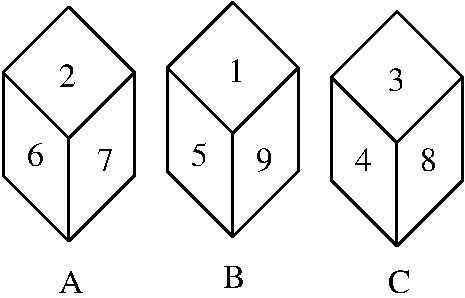
\includegraphics{dice.jpg}
\end{center}
In lecture we proved that if we roll each die once, then die $A$ beats $B$ more often, die $B$ beats die $C$ more often, and die $C$ beats die $A$ more often. Thus, contrary to our intuition, the ``beats'' relation $>$ is not transitive. That is, we have $A > B > C > A$.

We then looked at what happens if we roll each die twice, and add the result. We will show that the ``beats'' relation reverses in this game, that is, $A < B < C < A$, which is very counterintuitive!

\bparts

\ppart{5}
Show that rolling die $C$ twice is more likely to win than rolling die $B$ twice.

\solution{We draw the sample space. In the figure, it should be understood that the tree corresponding to $B$ is connected to each leaf of the tree corresponding to $C$. 
\begin{center}
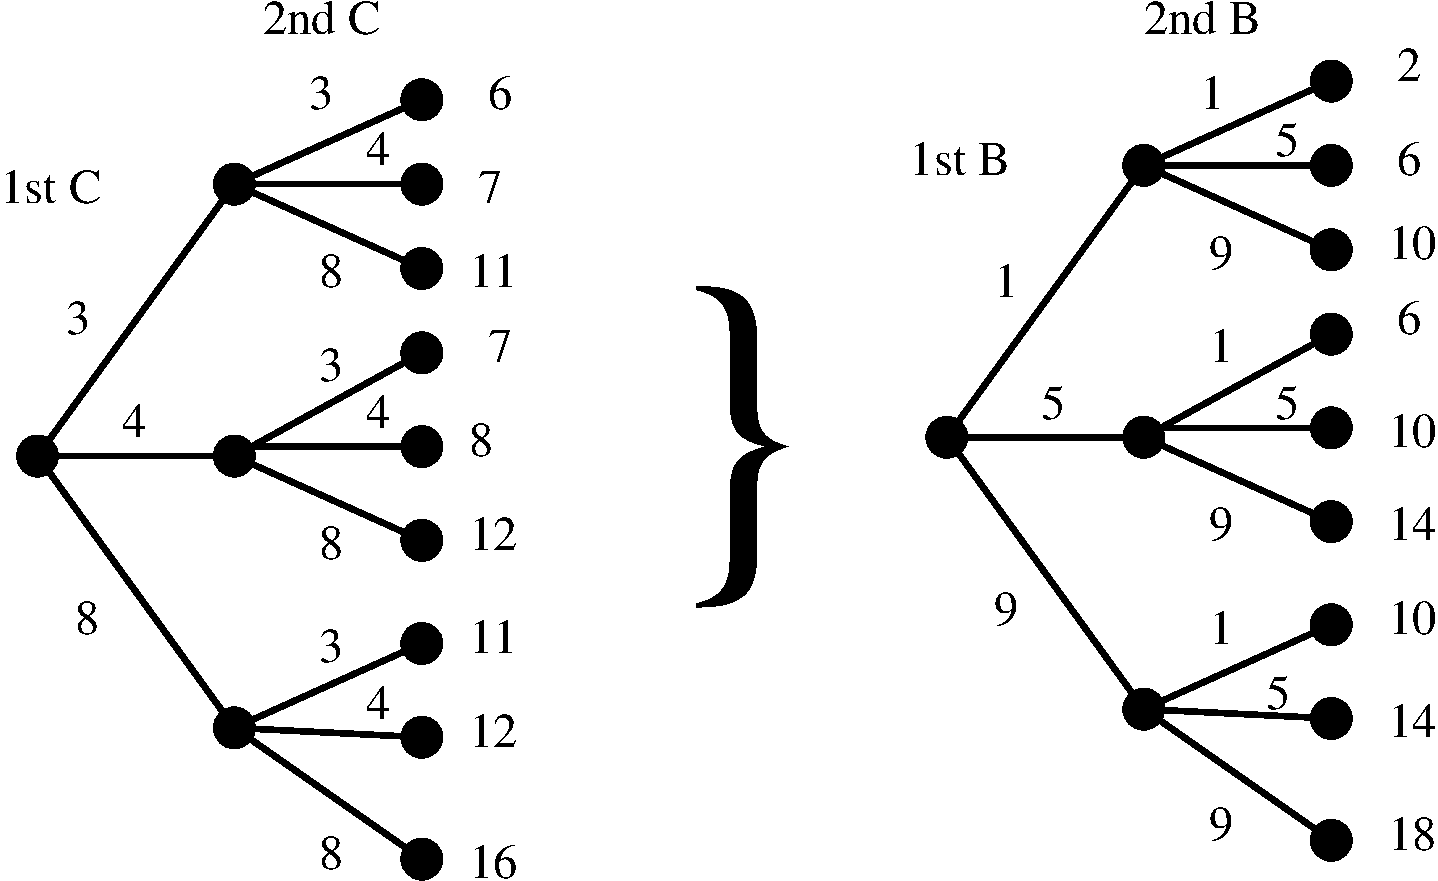
\includegraphics{dieSum2.jpg}
\end{center}

As in lecture, there are $81$ leaves and the space is uniform, i.e., each outcome occurs with probability $(1/3)^4 = 1/81$. Let's work out the chances of winning. The sum of the two rolls of the $B$ die is equally likely to be any element of the following multiset:
$$S_B = \{2, 6, 6, 10, 10, 10, 14, 14, 18\}.$$
The sum of the two rolls of the $C$ die is equally likely to be any element of the following multiset:
$$S_C = \{6, 7, 7, 8, 11, 11, 12, 12, 16\}.$$
We can treat each outcome as a pair $(x,y) \in S_B \times S_C$, where $C$ wins iff $y > x$. If $y = 6$, there is $1$ value of $x$, namely $x = 2$, for which $y > x$. Continuing the count in this way, the number of pairs for which $y > x$ is $$1 + 3 + 3 + 3 + 6 + 6 + 6 + 6 + 8 = 42,$$
while there are $2$ ties and $37$ cases where $B$ wins. Thus, rolling die $C$ twice is more likely to win than rolling die $B$ twice.
}

\ppart{5} Show that rolling die $A$ twice is more likely to win that rolling die $C$ twice.

\solution{We draw the sample space. In the figure, it should be understood that the tree corresponding to $C$ is connected to each leaf of the tree corresponding to $A$. 
\begin{center}
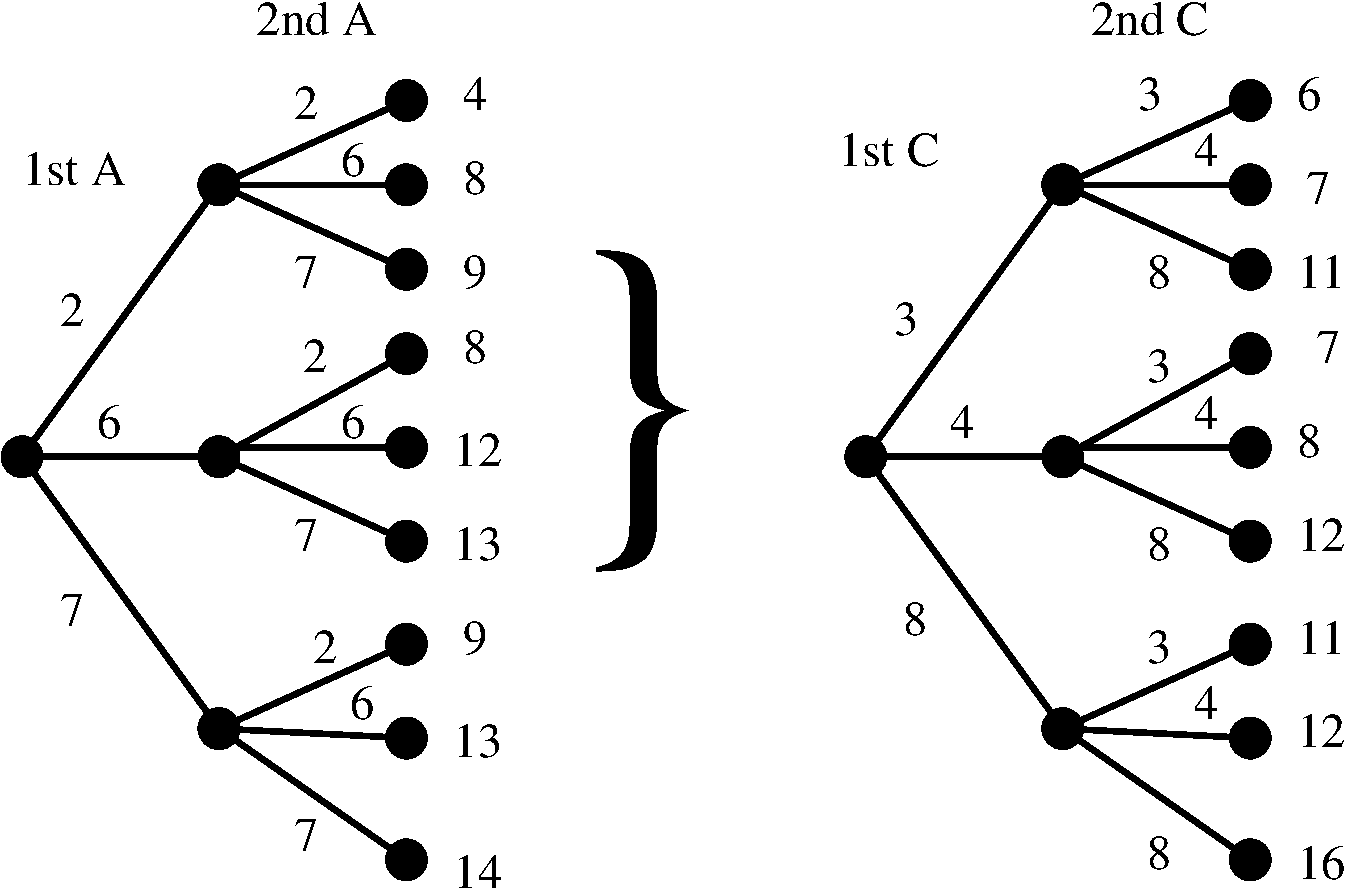
\includegraphics{dieSum3}
\end{center}
As in lecture, there are $81$ leaves and the space is uniform, i.e., each outcome occurs with probability $(1/3)^4 = 1/81$. Let's work out the chances of winning. The sum of the two rolls of the $C$ die is equally likely to be any element of the following multiset:
$$S_C = \{6, 7, 7, 8, 11, 11, 12, 12, 16\}.$$
The sum of the two rolls of the $A$ die is equally likely to be any element of the following multiset:
$$S_A = \{4, 8, 8, 9, 9, 12, 13, 13, 14\}.$$
We can treat each outcome as a pair $(x,y) \in S_C \times S_A$, where $A$ wins iff $y > x$. If $y = 4$, there is no $x$ for which $y > x$. If $y = 8$, there are $3$ values of $x$, namely $x = 6, 7, 7$, for which $y > x$. Continuing the count in this way, the number of pairs for which $y > x$ is $$0 + 3 + 3 + 4 + 4 + 6 + 8 + 8 + 8 = 44,$$
while a similar count shows that there are only $33$ pairs for which $x > y$, and there are $4$ ties. Thus, rolling die $A$ twice is more likely to win than rolling die $C$ twice.
}

\ppart{5}
Show that rolling die $B$ twice is more likely to win than rolling die $A$ twice.

\eparts 

\end{problem}



%%%%%%%%%%%%%%%%%%%%%%%%%%%%%%%%%%%%%%%%%%%%%%%%%%%%%%%%%%%%%%%%%%%%%%%%%%%%%
%%% Fall07 ps10 problem 3

\begin{problem}{14}
Let's play a game!  We repeatedly flip a fair coin.  You have the
sequence $HHT$, and I have the sequence $HTT$.  If your sequence comes
up first, then you win.  If my sequence comes up first, then I win.
For example, if the sequence of tosses is:
\[
TTHTHT\underline{HHT}
\]
then you win.  What is the probability that you win?  It may come as a
surprise that the answer is very different from 1/2.

This problem is tricky, because the game could go on for an arbitrarily
long time.  Draw enough of the tree diagram to see a pattern, and then sum
up the probabilities of the (infinitely many) outcomes in which you win.

It turns out that for any sequence of three flips, there is another
sequence that is likely to come up before it.  So there is no sequence
which turns up earliest! \dots and given any sequence, knowing how to pick
another sequence that comes up sooner more than half the time gives you a
nice chance to fool people gambling at a bar :-)


\solution{A partial tree diagram is shown below.  All edge
probabilities are $1/2$.

\bigskip
\centerline{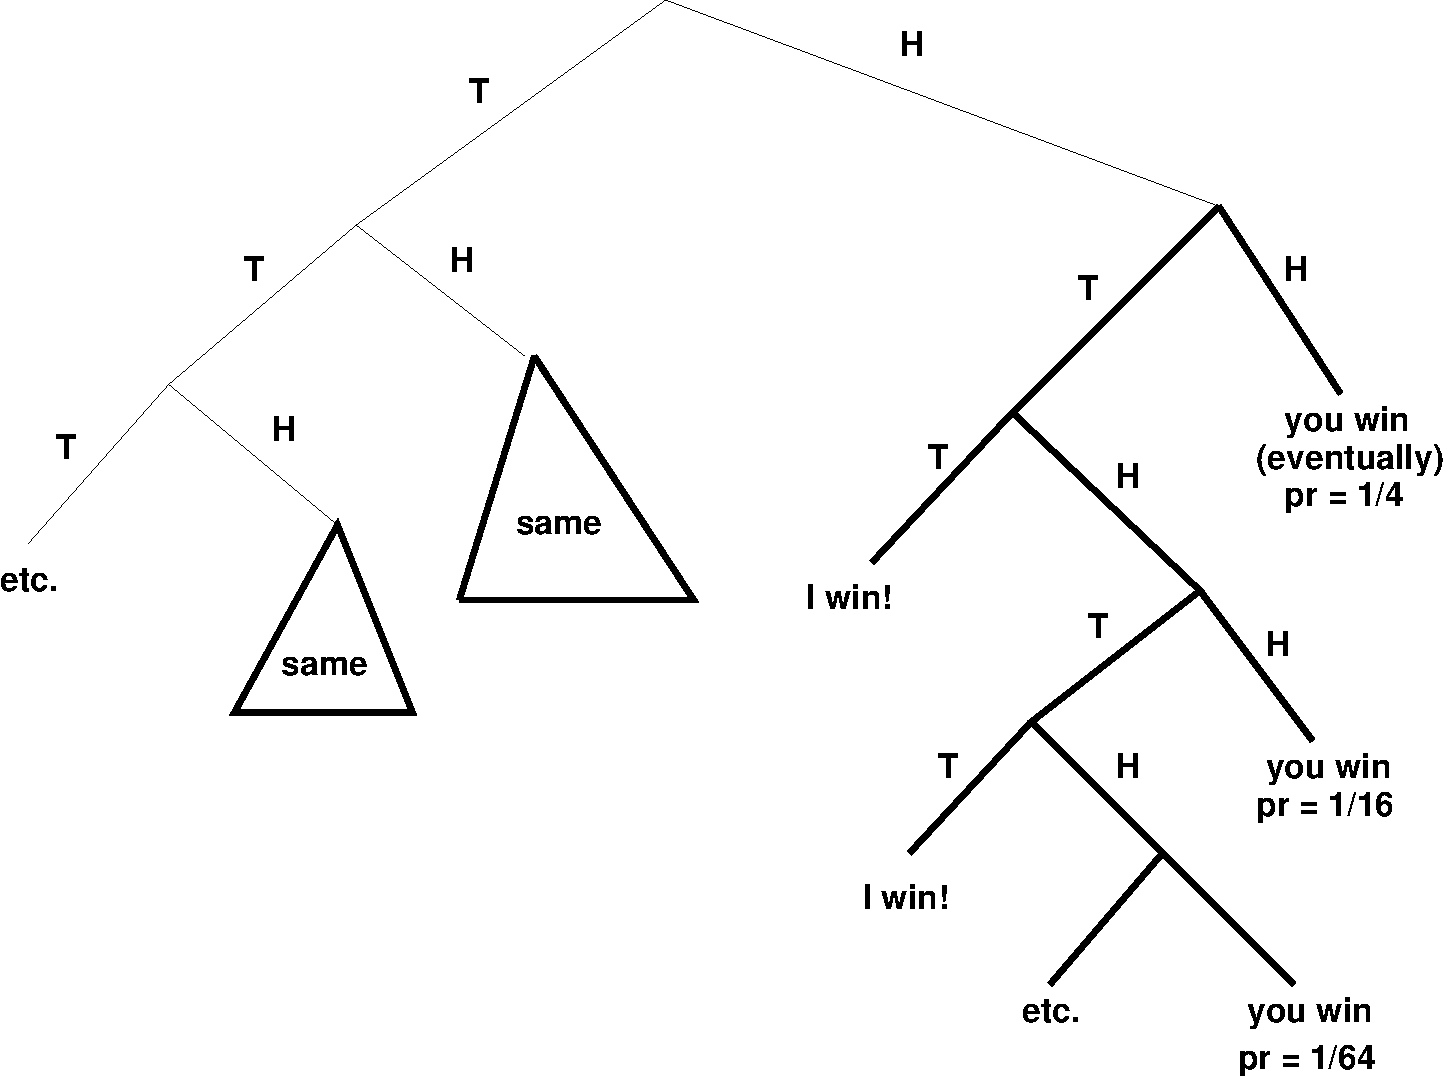
\includegraphics[height=3in]{ps9-HHTtree}}
\bigskip

Let's first focus on the subtree shown in bold.  Note that if two
heads are flipped in a row, then you are guaranteed to win eventually.
The sum of the probabilities of all your winning outcomes in this
subtree is:

\begin{eqnarray*}
\frac{1}{4} + \frac{1}{16} + \frac{1}{64} + \ldots
	& = & \frac{1}{4} \cdot \frac{1}{1 - 1/4} \\
	& = & \frac{1}{3}
\end{eqnarray*}

The uppermost subtree marked {\bf same} is identical to the one
shown in bold, except that each outcome probability is reduced by
$1/2$, because it is one edge farther from the root.  Thus, the sum of
your winning outcomes in this subtree is $1/6$.  Similarly, the sum of
your winning outcomes in the next subtree marked {\bf same} is $1/12$,
and so forth.  Overall, your probability of winning is:

\begin{eqnarray*}
\frac{1}{3} + \frac{1}{6} + \frac{1}{12} + \ldots
	& = & \frac{1}{3} \cdot \frac{1}{1 - 1/2} \\
	& = & \frac{2}{3}
\end{eqnarray*}
}

\end{problem}



\begin{problem}{15}
We're interested in the probability that a randomly chosen poker hand (5
cards from a standard 52-card deck) contains cards from at most two suits.

\bparts

\ppart{7} What is an appropriate sample space to use for this problem?  What
are the outcomes in the event, $\cE$, we are interested in?  What are the
probabilities of the individual outcomes in this sample space?

\solution{The natural sample space to use consists of the $\binom{52}{5}$ possible poker hands. We define $\cE$ to be the subset of outcomes in which the 5 cards on the outcome come from at most two suits. The sample space is \emph{uniform}: Each hand is equally likely and comes up with probability $1 / \binom{52}{5}$.}

\ppart{8}  What is $\prob{\cE}$?

\solution{Since the sample space is uniform,
\[
\prob{\cE} = \frac{\card{\cE}}{\dbinom{52}{5}}.
\]
We can count the size of $\cE$ by cases. There are three cases: five cards of the same suit; four cards of one suit and one of another; and three cards of one suit and two of another.

For five of one suit, there are 4 ways to choose the suit and then
$\binom{13}{5}$ ways to choose 5 cards from that suit.

For four of one suit and one of another, there are 4 ways to choose the larger suit and $\binom{13}{4}$ ways to choose 4 cards from that suit. Then there are 3 remaining suits from which to choose 1, and 13 choices for the 1 card of that suit.

Finally, for 3 of one suit and 2 of another, there are 4 ways to choose
the suit of 3 and $\binom{13}{3}$ ways to choose cards for that suit,
and there are 3 remaining suits to choose for the 2 cards, and
$\binom{13}{2}$ choices for the 2 cards of that suit. So the total is
\[
4\cdot \binom{13}{5} + 4 \cdot \binom{13}{4} \cdot 3 \cdot 13 + 4 \cdot
\binom{13}{3} \cdot 3 \cdot \binom{13}{2},
\]
and the probability of at most two suits 
is
\[
\frac{4\cdot \dbinom{13}{5} + 4 \cdot \dbinom{13}{4} \cdot 3 \cdot 13 + 4 \cdot
\dbinom{13}{3} \cdot 3 \cdot \dbinom{13}{2}}{\dbinom{52}{5}}
 = 88/595 \approx 0.15.
\]
}
\eparts

\end{problem}

%%%%%%%%%%%%%%%%%%%%%%%%%%%%%%%%%%%%%%%%%%%%%%%%%%%%%%%%%%%%%%%%%%%%%%%%%%%%%%

\begin{problem}{21}

  I have a deck of $52$ regular playing cards, $26$ red, $26$ black,
  randomly shuffled.  They all lie face down in the deck so that you
  can't see them.  I will draw a card off the top of the deck and turn
  it face up so that you can see it and then put it aside. I will
  continue to turn up cards like this but at some point while there
  are still cards left in the deck, you have to declare that you want
  the next card in the deck to be turned up.  If that next card turns
  up black you win and otherwise you lose.  Either way, the game is
  then over.

\bparts

\ppart{4} Show that if you take the first card before you have seen any
cards, you then have probability $1/2$ of winning the game.

\solution{If we just record the sequence of black and red cards that
  will be drawn, there are $\binom{51}{25}$ sequences with first card
  black: $25$ positions for the black cards chosen from the $51$
  remaining positions.  Since there are $\binom{52}{26}$ sequences in
  all, the probability of winning on the first draw is
  $\binom{51}{25}/\binom{52}{26} = 26/52 = 1/2$.}

\ppart{4} Suppose you don't take the first card and it turns up red.
Show that you have then have a probability of winning the game that is
greater than $1/2$.

\solution{Suppose you take the next card after that.  There are
  $\binom{50}{25}$ sequences that start with a red card and then a
  black and there are $\binom{51}{26}$ sequences that start with a red
  card. So then there is a $\binom{50}{25}/\binom{50}{26} = 26/51 >
  1/2$ chance of winning.  Any optimum strategy would have to
  guarantee a probability of winning as least as big as that.}

\ppart{4} If there are $r$ red cards left in the deck and $b$ black
cards, show that the probability of winning in you take the next card
is $b/(r+b)$.

\solution{The probability is $\binom{b+r-1}{b-1}/\binom{b+r}{b} =
b/(r+b)$.}

\ppart{9} Either,
\begin{enumerate}
\item come up with a strategy for this game that gives you a
  probability of winning strictly greater than $1/2$ and prove that
  the strategy works, or,
\item come up with a proof that no such strategy can exist.
\end{enumerate}

\solution{There is no such strategy.  Let $S_{b,r}$ be a strategy that
  acchieves the best probability of winning when starting with $b$
  black cards and $r$ red cards.  The claim is that $\Pr(\mbox{win by
    playing $S_{b,r}$}) = b/(r+b)$ for all $b,r$ with at least $b>0$
  or $r>0$.

  Clearly $\Pr(\mbox{win by playing $S_{1,0}$}) = 1$ and
  $\Pr(\mbox{win by playing $S_{0,1}$}) = 0$. We prove the rest of the
  claim by induction on $r+b$.  If the strategy $S_{b,r}$ is to take
  the next card, then $\Pr(\mbox{win by playing $S_{b,r}$}) = b/(r+b)$
  as claimed.  Suppose then that the strategy $S_{r,b}$ is to not take
  the first card, but to keep playing. Then by the law of total
  probability,
  \[\Pr(\mbox{win by playing $S_{b,r}$}) = \Pr(\mbox{win by
    playing $S_{b,r}$} |\mbox{first card is black}) \Pr(\mbox{first
    card is black})\] \[ +\Pr(\mbox{win by playing
    $S_{b,r}$}|\mbox{first card is red}) \Pr(\mbox{first card is
    red})\]
  \[ = Pr(\mbox{win by playing $S_{b-1,r}$}) (b/(r+b)) + \Pr(\mbox{win
    by playing $S_{b,r-1}$})(r/(b+r)).\]  By induction, this is
  \[\Pr(\mbox{win by playing $S_{b,r}$}) = ((b-1)/(b-1+r))(b/(r+b)) +
  (b/(b+r-1))(r/(b+r)) = b/(b+r),\] as claimed.  Why is $\Pr(\mbox{win
    by playing $S_{b,r}$} |\mbox{first card is black}) = Pr(\mbox{win by
    playing $S_{b-1,r}$})$?  If you have decided to see at least one
  more card, and that card is black, this means you are starting the
  game over again with $S_{b-1,r}$.}

\eparts

\end{problem}




\end{document}
